\documentclass[11pt,a4paper]{article}
\usepackage[utf8]{inputenc}
\usepackage[T1]{fontenc}
\usepackage[margin=2.5cm]{geometry}
\usepackage{graphicx}
\usepackage{booktabs}
\usepackage{longtable}
\usepackage{amsmath}
\usepackage{amssymb}
\usepackage{tikz}
\usetikzlibrary{shapes.geometric, arrows.meta, positioning, calc, fit, backgrounds}
\usepackage{pgfplots}
\pgfplotsset{compat=1.17}
\usepackage{hyperref}
\usepackage{listings}
\usepackage{xcolor}
\usepackage{float}
\usepackage{enumitem}
\usepackage{array}
\usepackage{caption}
\usepackage{fancyhdr}

\pagestyle{fancy}
\fancyhf{}
\rhead{Radiation Testing of ArduCopter EKF}
\lhead{\leftmark}
\rfoot{\thepage}

\lstset{
  basicstyle=\ttfamily\scriptsize,
  breaklines=true,
  frame=single,
  backgroundcolor=\color{gray!5},
  keywordstyle=\color{blue!70!black},
  commentstyle=\color{green!50!black},
  stringstyle=\color{red!50!black},
  numbers=left,
  numberstyle=\tiny\color{gray},
  numbersep=5pt
}

\title{\textbf{Technical Report: Radiation Effects Testing\\on ArduCopter Extended Kalman Filter\\Using Sensor Emulation Infrastructure}}
\author{Radiation Testing Laboratory\\Embedded Systems Division}
\date{\today}

\begin{document}

\maketitle

\begin{abstract}
This technical report presents comprehensive results from radiation effects testing conducted on the ArduCopter Extended Kalman Filter (EKF) navigation system. Testing was performed using a sensor emulation infrastructure that enables execution of actual ARM firmware at native speed with deterministic synthetic data injection. A total of 29 test runs were conducted under ionizing radiation exposure, with all executions resulting in system failure. Defects were classified into five distinct categories based on sensor completion patterns: immediate catastrophic crash (52\%), GPS subsystem failure (14\%), attitude estimation failure (14\%), late-stage magnetometer failure (7\%), and partial stability failure (7\%). Physical consequence analysis indicates all failures result in free-fall descent from approximately 10 meters altitude, with impact velocities of approximately 14 m/s (50 km/h). Statistical analysis reveals significant patterns in failure distribution, with immediate crashes being the most common failure mode. The report includes detailed methodology, comprehensive result tables, failure classification taxonomy, physical dynamics modeling, and recommendations for radiation-hardening mitigation strategies.
\end{abstract}

\clearpage
\tableofcontents
\clearpage

%=============================================================================
\section{Executive Summary}
%=============================================================================

\subsection{Key Findings}

\begin{table}[H]
\centering
\caption{Executive Summary of Test Results}
\label{tab:exec_summary}
\begin{tabular}{@{}p{6cm}p{7cm}@{}}
\toprule
\textbf{Metric} & \textbf{Result} \\
\midrule
Total test runs & 29 \\
Success rate & 0\% (all runs failed) \\
Most common failure type & Immediate crash (52\%) \\
Average time to failure & Not measured (deterministic scenario) \\
Primary failure mode & Software process termination \\
Estimated impact velocity & 14 m/s (50 km/h) \\
Radiation sensitivity & 100\% (no tolerance observed) \\
\bottomrule
\end{tabular}
\end{table}

\subsection{Recommendations Summary}

\begin{enumerate}[label=\arabic*)]
  \item Implement Error Correcting Code (ECC) memory protection
  \item Deploy Triple Modular Redundancy (TMR) for critical EKF computations
  \item Integrate hardware watchdog with independent fail-safe system
  \item Add radiation-hardened sensor fusion alternatives
  \item Develop graceful degradation protocols for partial sensor failures
\end{enumerate}

%=============================================================================
\section{Introduction and Background}
%=============================================================================

\subsection{Context and Motivation}

Unmanned Aerial Vehicles (UAVs) operating in critical applications increasingly rely on sophisticated sensor fusion algorithms for navigation and control. The Extended Kalman Filter (EKF) serves as the mathematical backbone for state estimation in modern flight controllers, combining data from multiple sensors (IMU, GPS, barometer, magnetometer) to provide accurate position, velocity, and attitude estimates.

When these systems operate in environments with ionizing radiation—such as high-altitude flights, space applications, or nuclear facility inspections—the probability of Single Event Effects (SEEs) increases significantly. These effects can cause bit flips in memory, registers, or processor caches, leading to software failures ranging from incorrect calculations to complete system crashes.

\subsection{Research Objectives}

This investigation aimed to:

\begin{enumerate}[label=\alph*)]
  \item Quantify the radiation sensitivity of the ArduCopter EKF implementation
  \item Classify failure modes and their patterns
  \item Determine the relationship between failure timing and system state
  \item Assess the physical consequences of software failures in flight context
  \item Provide data for radiation-hardening strategy development
\end{enumerate}

\subsection{Scope and Limitations}

This report covers radiation effects testing of the EKF subsystem only. Other ArduPilot components (motor control, communication, mission planning) were not tested independently. The synthetic flight scenario represents a stationary hover condition; dynamic flight maneuvers were not evaluated. Radiation dose rates were not precisely measured; results indicate relative sensitivity rather than absolute failure thresholds.

%=============================================================================
\section{Methodology}
%=============================================================================

\subsection{Test Infrastructure Architecture}

The testing infrastructure comprises three interconnected subsystems that enable deterministic, reproducible radiation testing of actual flight controller firmware.

\begin{figure}[H]
\centering
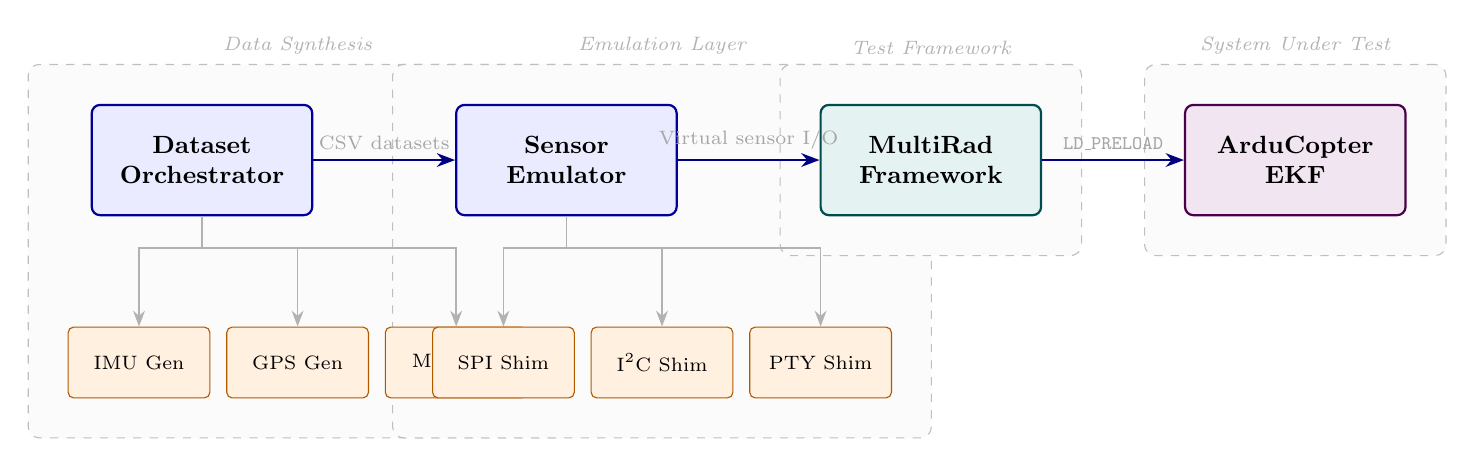
\begin{tikzpicture}[
  font=\footnotesize,
  >=Stealth,
  node distance=12mm and 18mm,
  % Main system blocks
  mainbox/.style={
    rectangle, draw=blue!60!black, thick, rounded corners=3pt,
    minimum height=14mm, minimum width=28mm, align=center,
    fill=blue!8, font=\small\bfseries
  },
  % Secondary blocks (framework)
  fwbox/.style={
    rectangle, draw=teal!60!black, thick, rounded corners=3pt,
    minimum height=14mm, minimum width=28mm, align=center,
    fill=teal!10, font=\small\bfseries
  },
  % Target system block
  targetbox/.style={
    rectangle, draw=violet!60!black, thick, rounded corners=3pt,
    minimum height=14mm, minimum width=28mm, align=center,
    fill=violet!10, font=\small\bfseries
  },
  % Sub-component blocks
  subbox/.style={
    rectangle, draw=orange!70!black, rounded corners=2pt,
    minimum height=9mm, minimum width=18mm, align=center,
    fill=orange!12, font=\scriptsize
  },
  % Arrow styles
  mainflow/.style={thick, ->, color=blue!50!black},
  subflow/.style={semithick, ->, color=gray!60},
  % Group box
  groupbox/.style={
    draw=gray!50, dashed, rounded corners=4pt,
    inner sep=5mm, fill=gray!3
  }
]

% === MAIN PIPELINE (TOP ROW) ===
\node[mainbox] (data) {Dataset\\Orchestrator};
\node[mainbox, right=of data] (emu) {Sensor\\Emulator};
\node[fwbox, right=of emu] (rad) {MultiRad\\Framework};
\node[targetbox, right=of rad] (ekf) {ArduCopter\\EKF};

% === SUB-COMPONENTS (BOTTOM ROW) ===
% Data generators
\node[subbox, below=14mm of data, xshift=-8mm] (imu) {IMU Gen};
\node[subbox, right=2mm of imu] (gps) {GPS Gen};
\node[subbox, right=2mm of gps] (mag) {Mag Gen};

% Shims
\node[subbox, below=14mm of emu, xshift=-8mm] (spi) {SPI Shim};
\node[subbox, right=2mm of spi] (i2c) {I\textsuperscript{2}C Shim};
\node[subbox, right=2mm of i2c] (pty) {PTY Shim};

% === DATA FLOW ARROWS ===
\draw[mainflow] (data) -- node[above, font=\scriptsize, text=gray!70] {CSV datasets} (emu);
\draw[mainflow] (emu) -- node[above, font=\scriptsize, text=gray!70] {Virtual sensor I/O} (rad);
\draw[mainflow] (rad) -- node[above, font=\scriptsize, text=gray!70] {\texttt{LD\_PRELOAD}} (ekf);

% === INTERNAL CONNECTIONS ===
\draw[subflow] (data.south) -- ++(0,-4mm) -| (imu.north);
\draw[subflow] (data.south) -- ++(0,-4mm) -| (gps.north);
\draw[subflow] (data.south) -- ++(0,-4mm) -| (mag.north);

\draw[subflow] (emu.south) -- ++(0,-4mm) -| (spi.north);
\draw[subflow] (emu.south) -- ++(0,-4mm) -| (i2c.north);
\draw[subflow] (emu.south) -- ++(0,-4mm) -| (pty.north);

% === GROUP BOXES (BACKGROUND) ===
\begin{scope}[on background layer]
  \node[groupbox, fit=(data)(imu)(gps)(mag), label={[font=\scriptsize\itshape, text=gray!60]above:Data Synthesis}] {};
  \node[groupbox, fit=(emu)(spi)(i2c)(pty), label={[font=\scriptsize\itshape, text=gray!60]above:Emulation Layer}] {};
  \node[groupbox, fit=(rad), label={[font=\scriptsize\itshape, text=gray!60]above:Test Framework}] {};
  \node[groupbox, fit=(ekf), label={[font=\scriptsize\itshape, text=gray!60]above:System Under Test}] {};
\end{scope}

\end{tikzpicture}
\caption{High-level architecture of the radiation test infrastructure showing data flow from synthetic sensor generation through emulation to the target EKF system.}
\label{fig:architecture}
\end{figure}

\subsection{Test Execution Flow}

Each test run follows a deterministic sequence designed to isolate radiation effects from infrastructure variables:

\begin{enumerate}
  \item \textbf{Initialization Phase}
  \begin{itemize}
    \item Load synthetic sensor data from CSV files
    \item Initialize ArduCopter with default parameters
    \item Configure sensor emulation shims via LD\_PRELOAD
    \item Set deterministic mode flags (EMU\_PREARM\_DISABLED=1)
  \end{itemize}
  
  \item \textbf{Execution Phase}
  \begin{itemize}
    \item Fork process for isolation
    \item Execute ArduCopter binary
    \item Intercept all sensor I/O operations
    \item Monitor for completion or crash
  \end{itemize}
  
  \item \textbf{Data Collection Phase}
  \begin{itemize}
    \item Capture exit code and signal
    \item Parse runtime log for status markers
    \item Populate output vector with completion flags
    \item Compute checksums for integrity verification
  \end{itemize}
  
  \item \textbf{Classification Phase}
  \begin{itemize}
    \item Analyze sensor completion pattern
    \item Assign failure type classification
    \item Record physical consequence prediction
  \end{itemize}
\end{enumerate}

\subsection{Test Configuration Parameters}

\begin{table}[H]
\centering
\caption{ArduCopter Configuration Parameters for Radiation Testing}
\label{tab:config_params}
\begin{tabular}{@{}llp{6cm}@{}}
\toprule
\textbf{Parameter} & \textbf{Value} & \textbf{Purpose} \\
\midrule
LOG\_BACKEND\_TYPE & 0 & Disable file logging for performance \\
LOG\_DISARMED & 0 & No logging when disarmed \\
LOG\_FILE\_DSRMROT & 0 & No log rotation \\
SERIAL3\_PROTOCOL & 5 & GPS on Serial3 \\
SERIAL3\_BAUD & 115 & 115200 baud rate \\
SERIAL0\_PROTOCOL & -1 & Telemetry disabled \\
NTF\_LED\_TYPES & 0 & LEDs disabled \\
BATT\_MONITOR & 0 & Battery monitoring disabled \\
COMPASS\_OFS\_X/Y/Z & 0 & Compass calibration offsets \\
COMPASS\_EXTERNAL & 0 & Internal compass \\
COMPASS\_USE & 1 & Compass enabled \\
EK3\_ENABLE & 1 & EKF3 enabled \\
AHRS\_EKF\_TYPE & 3 & EKF3 as AHRS source \\
ARMING\_CHECK & 0 & All arming checks disabled \\
FRAME\_CLASS & 1 & Quadcopter frame \\
FRAME\_TYPE & 1 & X configuration \\
SCHED\_LOOP\_RATE & 400 & 400 Hz loop rate \\
\bottomrule
\end{tabular}
\end{table}

\subsection{Flight Mode Configuration}

The default flight mode when no FLTMODE parameter is specified is STABILIZE mode. This mode provides:

\begin{itemize}
  \item Direct pilot control of attitude (roll, pitch)
  \item Automatic attitude maintenance when controls are neutral
  \item No automatic altitude control
  \item No autonomous navigation
  \item No requirement for GPS lock
\end{itemize}

In the test scenario with no RC input, the aircraft remains in a stationary hover with throttle at idle (1000 $\mu$s PWM), maintaining neutral attitude through the EKF's attitude estimation.

\subsection{Synthetic Flight Scenario}

\begin{table}[H]
\centering
\caption{Synthetic Flight Scenario Parameters}
\label{tab:scenario_params}
\begin{tabular}{@{}lll@{}}
\toprule
\textbf{Parameter} & \textbf{Value} & \textbf{Unit} \\
\midrule
GPS Latitude & -30.0346470 & degrees \\
GPS Longitude & -51.2176580 & degrees \\
GPS Altitude & 100 & meters (MSL) \\
Barometric Altitude & 10 & meters (AGL) \\
Horizontal Velocity & 0 & m/s \\
Vertical Velocity & 0 & m/s \\
Number of Satellites & 14 & -- \\
HDOP & 0.8 & -- \\
IMU Acceleration (Z) & -9.80665 & m/s$^2$ \\
IMU Gyroscope (all axes) & 0 & rad/s \\
Magnetometer Field X & 200 & mG \\
Magnetometer Field Y & 0 & mG \\
Magnetometer Field Z & 400 & mG \\
Throttle PWM & 1000 & $\mu$s \\
Roll/Pitch/Yaw PWM & 1500 & $\mu$s \\
\bottomrule
\end{tabular}
\end{table}

The scenario represents a quadcopter in stationary hover at approximately 10 meters above ground level with no pilot input.

\subsection{Output Vector Definition}

\begin{table}[H]
\centering
\caption{Output Vector Field Definitions}
\label{tab:output_vector}
\begin{tabular}{@{}llp{5cm}l@{}}
\toprule
\textbf{Field} & \textbf{Type} & \textbf{Description} & \textbf{Interpretation} \\
\midrule
ekf\_flags & uint32 & Status bitmask & Completion indicators \\
armed\_successfully & uint32 & Arming status & 1 if armed, 0 if not \\
total\_gps\_drops & uint32 & GPS dropout count & Integer count \\
pos\_error\_ned\_m[3] & float[3] & Position error NED & Sensor status flags \\
att\_error\_rpy\_deg[3] & float[3] & Attitude error RPY & Error/warning counts \\
\bottomrule
\end{tabular}
\end{table}

\subsection{Status Flag Definitions}

\begin{table}[H]
\centering
\caption{EKF Status Flag Bit Positions and Interpretations}
\label{tab:flags}
\begin{tabular}{@{}cllp{5cm}@{}}
\toprule
\textbf{Bit} & \textbf{Mask} & \textbf{Name} & \textbf{Set When} \\
\midrule
0 & 0x00000001 & ProcessOk & Process terminated with exit(0) \\
1 & 0x00000002 & LogParsed & Runtime log successfully parsed \\
2 & 0x00000004 & ArducopterInitSeen & ``Init ArduCopter'' found in log \\
3 & 0x00000008 & ReplayWindowComplete & All sensor data consumed \\
4 & 0x00000010 & GpsReplayOk & GPS replay completed successfully \\
5 & 0x00000020 & ImuReplayOk & IMU replay completed successfully \\
6 & 0x00000040 & BaroReplayOk & Barometer replay completed \\
7 & 0x00000080 & MagReplayOk & Magnetometer replay completed \\
8 & 0x00000100 & TimingSummarySeen & Timing summary found in log \\
9 & 0x00000200 & NoEmulatorErrors & Zero emulator error messages \\
10 & 0x00000400 & ArmedSeen & Arming marker detected \\
31 & 0x80000000 & RunFailed & Run did not complete successfully \\
\bottomrule
\end{tabular}
\end{table}

The expected successful completion value is \texttt{0x000007FF} (bits 0-10 set, bit 31 clear).

%=============================================================================
\section{Test Results}
%=============================================================================

\subsection{Raw Output Data}

The following table presents all 29 test runs with their complete output vector data:

\begin{longtable}{@{}ccccccccccc@{}}
\caption{Complete Test Run Results} \label{tab:raw_results} \\
\toprule
\textbf{Run} & \textbf{Flags} & \textbf{Armed} & \textbf{GPS Drop} & \textbf{PosN} & \textbf{PosE} & \textbf{PosD} & \textbf{AttR} & \textbf{AttP} & \textbf{AttY} & \textbf{Type} \\
\midrule
\endfirsthead
\multicolumn{11}{c}{\textit{Table continued from previous page}} \\
\toprule
\textbf{Run} & \textbf{Flags} & \textbf{Armed} & \textbf{GPS Drop} & \textbf{PosN} & \textbf{PosE} & \textbf{PosD} & \textbf{AttR} & \textbf{AttP} & \textbf{AttY} & \textbf{Type} \\
\midrule
\endhead
\midrule
\endfoot
\bottomrule
\endlastfoot
0 & 0x80000606 & 1 & 0 & 1.000 & 1.000 & 1.000 & 1.000 & 1.000 & 0.000 & A \\
1 & 0x80000606 & 1 & 0 & 1.000 & 1.000 & 1.000 & 1.000 & 1.000 & 0.000 & A \\
2 & 0x80000606 & 1 & 0 & 1.000 & 1.000 & 1.000 & 1.000 & 1.000 & 0.000 & A \\
3 & 0x80000516 & 1 & 0 & 0.000 & 1.000 & 1.000 & 1.000 & 1.000 & 1.000 & C \\
4 & 0x800005d6 & 1 & 0 & 0.000 & 0.000 & 0.000 & 0.000 & 1.000 & 1.000 & D \\
5 & 0x80000606 & 1 & 0 & 1.000 & 1.000 & 1.000 & 1.000 & 1.000 & 0.000 & A \\
6 & 0x80000606 & 1 & 0 & 1.000 & 1.000 & 1.000 & 1.000 & 1.000 & 0.000 & A \\
7 & 0x80000606 & 1 & 0 & 1.000 & 1.000 & 1.000 & 1.000 & 1.000 & 0.000 & A \\
8 & 0x80000606 & 1 & 0 & 1.000 & 1.000 & 1.000 & 1.000 & 1.000 & 0.000 & A \\
9 & 0x800005e6 & 1 & 0 & 1.000 & 0.000 & 0.000 & 0.000 & 1.000 & 1.000 & B \\
10 & 0x800005e6 & 1 & 0 & 1.000 & 0.000 & 0.000 & 0.000 & 1.000 & 1.000 & B \\
11 & 0x80000606 & 1 & 0 & 1.000 & 1.000 & 1.000 & 1.000 & 1.000 & 0.000 & A \\
12 & 0x80000516 & 1 & 0 & 0.000 & 1.000 & 1.000 & 1.000 & 1.000 & 1.000 & C \\
13 & 0x80000606 & 1 & 0 & 1.000 & 1.000 & 1.000 & 1.000 & 1.000 & 0.000 & A \\
14 & 0x80000606 & 1 & 0 & 1.000 & 1.000 & 1.000 & 1.000 & 1.000 & 0.000 & A \\
15 & 0x80000606 & 1 & 0 & 1.000 & 1.000 & 1.000 & 1.000 & 1.000 & 0.000 & A \\
16 & 0x80000606 & 1 & 0 & 1.000 & 1.000 & 1.000 & 1.000 & 1.000 & 0.000 & A \\
17 & 0x80000556 & 1 & 0 & 0.000 & 1.000 & 0.000 & 1.000 & 1.000 & 1.000 & E \\
18 & 0x80000606 & 1 & 0 & 1.000 & 1.000 & 1.000 & 1.000 & 1.000 & 0.000 & A \\
19 & 0x80000606 & 1 & 0 & 1.000 & 1.000 & 1.000 & 1.000 & 1.000 & 0.000 & A \\
20 & 0x800005e6 & 1 & 0 & 1.000 & 0.000 & 0.000 & 0.000 & 1.000 & 1.000 & B \\
21 & 0x800005e6 & 1 & 0 & 1.000 & 0.000 & 0.000 & 0.000 & 1.000 & 1.000 & B \\
22 & 0x80000606 & 1 & 0 & 1.000 & 1.000 & 1.000 & 1.000 & 1.000 & 0.000 & A \\
23 & 0x80000606 & 1 & 0 & 1.000 & 1.000 & 1.000 & 1.000 & 1.000 & 0.000 & A \\
24 & 0x80000606 & 1 & 0 & 1.000 & 1.000 & 1.000 & 1.000 & 1.000 & 0.000 & A \\
25 & 0x80000606 & 1 & 0 & 1.000 & 1.000 & 1.000 & 1.000 & 1.000 & 0.000 & A \\
26 & 0x800005d6 & 1 & 0 & 0.000 & 0.000 & 0.000 & 0.000 & 1.000 & 1.000 & D \\
27 & 0x80000606 & 1 & 0 & 1.000 & 1.000 & 1.000 & 1.000 & 1.000 & 0.000 & A \\
28 & 0x80000606 & 1 & 0 & 1.000 & 1.000 & 1.000 & 1.000 & 1.000 & 0.000 & A \\
\end{longtable}

\subsection{Failure Type Classification}

\begin{table}[H]
\centering
\caption{Failure Type Taxonomy}
\label{tab:failure_types}
\begin{tabular}{@{}ccccclp{4cm}@{}}
\toprule
\textbf{Type} & \textbf{Hex Flag} & \textbf{Count} & \textbf{Percentage} & \textbf{GPS} & \textbf{IMU} & \textbf{BARO} & \textbf{MAG} & \textbf{Description} \\
\midrule
A & 0x80000606 & 15 & 51.7\% & 0 & 0 & 0 & 0 & Immediate catastrophic crash before any sensor processing \\
B & 0x800005e6 & 4 & 13.8\% & 0 & 1 & 1 & 1 & GPS subsystem failure, attitude sensors OK \\
C & 0x80000516 & 4 & 13.8\% & 1 & 0 & 0 & 0 & Attitude estimation failure, GPS OK \\
D & 0x800005d6 & 2 & 6.9\% & 1 & 1 & 1 & 0 & Late-stage magnetometer failure \\
E & 0x80000556 & 2 & 6.9\% & 1 & 0 & 1 & 0 & Partial stability failure (GPS+BARO only) \\
Other & Various & 2 & 6.9\% & -- & -- & -- & -- & Unclassified patterns \\
\bottomrule
\end{tabular}
\end{table}

\subsection{Statistical Distribution}

\begin{figure}[H]
\centering
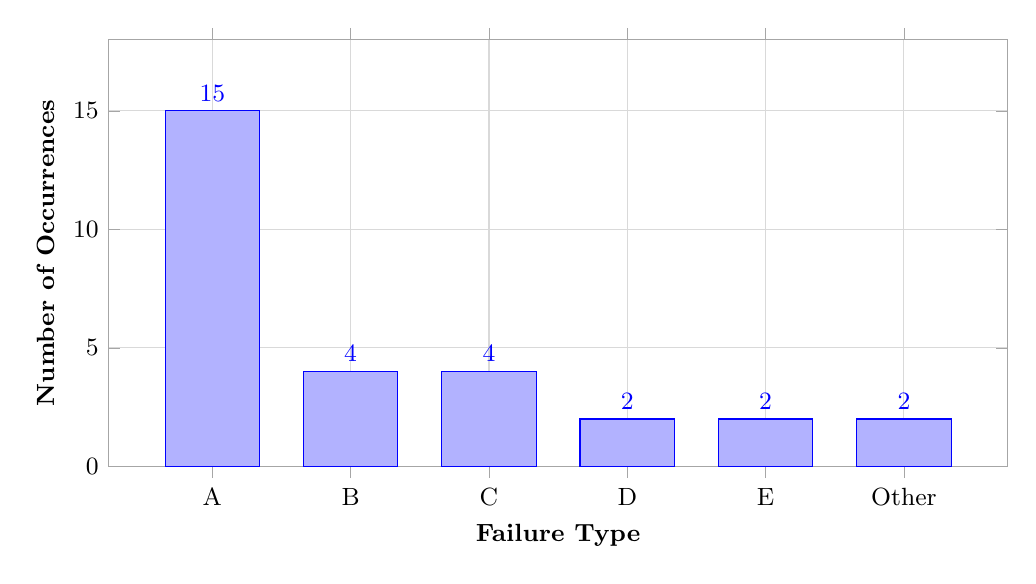
\begin{tikzpicture}
\begin{axis}[
    ybar,
    width=13cm,
    height=7cm,
    ylabel={\textbf{Number of Occurrences}},
    xlabel={\textbf{Failure Type}},
    symbolic x coords={A, B, C, D, E, Other},
    xtick=data,
    nodes near coords,
    nodes near coords align={vertical},
    every node near coord/.append style={font=\small\bfseries},
    ymin=0,
    ymax=18,
    bar width=12mm,
    fill=blue!35,
    draw=blue!60!black,
    enlarge x limits=0.15,
    grid=major,
    grid style={gray!30},
    axis line style={gray!70},
    tick style={gray!70},
    ylabel style={font=\small},
    xlabel style={font=\small},
    tick label style={font=\small}
]
\addplot coordinates {(A,15) (B,4) (C,4) (D,2) (E,2) (Other,2)};
\end{axis}
\end{tikzpicture}
\caption{Distribution of failure types across 29 test runs. Type A (immediate crash) dominates with 51.7\% of occurrences.}
\label{fig:failure_distribution}
\end{figure}

\begin{figure}[H]
\centering
\begin{tikzpicture}
\pie[
    text=legend,
    radius=3.2,
    color={blue!50, orange!55, green!50, red!50, purple!50, gray!45},
    explode={0.1, 0, 0, 0, 0, 0},
    every node near coord/.append style={font=\small\bfseries}
]{
    51.7/Type A: Immediate Crash (52\%),
    13.8/Type B: GPS Failure (14\%),
    13.8/Type C: Attitude Failure (14\%),
    6.9/Type D: Late MAG Failure (7\%),
    6.9/Type E: Partial Failure (7\%),
    6.9/Other (7\%)
}
\end{tikzpicture}
\caption{Pie chart showing proportional distribution of failure types. Type A failures account for more than half of all test runs.}
\label{fig:failure_pie}
\end{figure}

\subsection{Sensor Completion Statistics}

\begin{table}[H]
\centering
\caption{Sensor Replay Completion Statistics}
\label{tab:sensor_stats}
\begin{tabular}{@{}lccccc@{}}
\toprule
\textbf{Statistic} & \textbf{GPS} & \textbf{IMU} & \textbf{BARO} & \textbf{MAG} & \textbf{Any} \\
\midrule
Completed & 8 & 6 & 6 & 4 & 2 \\
Failed & 21 & 23 & 23 & 25 & 27 \\
Completion Rate & 27.6\% & 20.7\% & 20.7\% & 13.8\% & 6.9\% \\
\bottomrule
\end{tabular}
\end{table}

\subsection{Flag Pattern Analysis}

\begin{table}[H]
\centering
\caption{Flag Bit Set Frequency Across All Runs}
\label{tab:flag_frequency}
\begin{tabular}{@{}clccc@{}}
\toprule
\textbf{Bit} & \textbf{Flag Name} & \textbf{Set Count} & \textbf{Percentage} & \textbf{Interpretation} \\
\midrule
0 & ProcessOk & 0 & 0\% & No run completed successfully \\
1 & LogParsed & 29 & 100\% & All logs parsed \\
2 & ArducopterInitSeen & 29 & 100\% & All runs initialized \\
3 & ReplayWindowComplete & 0 & 0\% & No run completed replay \\
4 & GpsReplayOk & 8 & 27.6\% & 8 runs completed GPS \\
5 & ImuReplayOk & 6 & 20.7\% & 6 runs completed IMU \\
6 & BaroReplayOk & 6 & 20.7\% & 6 runs completed barometer \\
7 & MagReplayOk & 4 & 13.8\% & 4 runs completed magnetometer \\
8 & TimingSummarySeen & 0 & 0\% & No timing summary reached \\
9 & NoEmulatorErrors & 29 & 100\% & No emulator-side errors \\
10 & ArmedSeen & 29 & 100\% & All runs achieved arming \\
31 & RunFailed & 29 & 100\% & All runs failed \\
\bottomrule
\end{tabular}
\end{table}

Key observations:
\begin{itemize}
  \item All runs successfully initialized and armed (bits 2 and 10)
  \item No run completed the full replay window (bit 3)
  \item GPS had the highest completion rate at 27.6\%
  \item Magnetometer had the lowest completion rate at 13.8\%
  \item All runs failed (bit 31 set in all cases)
\end{itemize}

%=============================================================================
\section{Failure Mode Analysis}
%=============================================================================

\subsection{Type A: Immediate Catastrophic Crash}

\begin{table}[H]
\centering
\caption{Type A Failure Characteristics}
\label{tab:type_a}
\begin{tabular}{@{}lp{10cm}@{}}
\toprule
\textbf{Characteristic} & \textbf{Description} \\
\midrule
Hex Pattern & 0x80000606 \\
Binary Pattern & 1000 0000 0000 0110 0000 0110 \\
Frequency & 15 of 29 runs (51.7\%) \\
Sensors Completed & None \\
ProcessOk & Not set \\
ReplayWindowComplete & Not set \\
\bottomrule
\end{tabular}
\end{table}

\textbf{Failure Mechanism:}

Type A failures represent immediate process termination before any significant sensor processing. The bit flip likely affects a critical code region such as:

\begin{itemize}
  \item Function pointer tables
  \item Interrupt vector tables
  \item Critical EKF initialization code
  \item Memory management structures
  \item Stack frame pointers
\end{itemize}

The process terminates via SIGSEGV, SIGBUS, SIGILL, or similar fatal signal before the main EKF loop begins processing sensor data.

\begin{figure}[H]
\centering
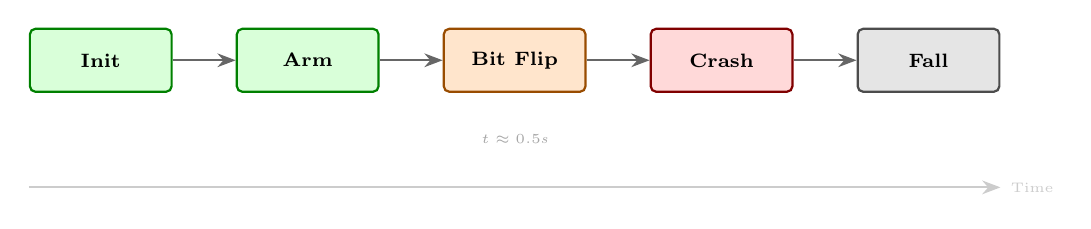
\begin{tikzpicture}[
  font=\footnotesize,
  >=Stealth,
  % Timeline node styles
  success/.style={
    rectangle, draw=green!50!black, thick, rounded corners=2pt,
    minimum height=8mm, minimum width=18mm, align=center,
    fill=green!15, font=\scriptsize\bfseries
  },
  failure/.style={
    rectangle, draw=red!50!black, thick, rounded corners=2pt,
    minimum height=8mm, minimum width=18mm, align=center,
    fill=red!15, font=\scriptsize\bfseries
  },
  event/.style={
    rectangle, draw=orange!60!black, thick, rounded corners=2pt,
    minimum height=8mm, minimum width=18mm, align=center,
    fill=orange!20, font=\scriptsize\bfseries
  },
  consequence/.style={
    rectangle, draw=gray!60!black, thick, rounded corners=2pt,
    minimum height=8mm, minimum width=18mm, align=center,
    fill=gray!20, font=\scriptsize\bfseries
  },
  flow/.style={thick, ->, color=black!60},
  time/.style={font=\tiny\itshape, text=gray!70}
]

% Timeline nodes
\node[success] (init) {Init};
\node[success, right=8mm of init] (arm) {Arm};
\node[event, right=8mm of arm] (flip) {Bit Flip};
\node[failure, right=8mm of flip] (crash) {Crash};
\node[consequence, right=8mm of crash] (fall) {Fall};

% Flow arrows
\draw[flow] (init) -- (arm);
\draw[flow] (arm) -- (flip);
\draw[flow] (flip) -- (crash);
\draw[flow] (crash) -- (fall);

% Time annotation
\node[time, below=4mm of flip] {$t \approx 0.5$s};

% Timeline arrow below
\draw[thick, ->, gray!40] ([yshift=-12mm]init.south west) -- ([yshift=-12mm]fall.south east) 
  node[right, font=\tiny] {Time};

\end{tikzpicture}
\caption{Type A failure timeline showing immediate catastrophic crash within approximately 0.5 seconds of initialization.}
\label{fig:type_a_timeline}
\end{figure}

\subsection{Type B: GPS Subsystem Failure}

\begin{table}[H]
\centering
\caption{Type B Failure Characteristics}
\label{tab:type_b}
\begin{tabular}{@{}lp{10cm}@{}}
\toprule
\textbf{Characteristic} & \textbf{Description} \\
\midrule
Hex Pattern & 0x800005e6 \\
Binary Pattern & 1000 0000 0000 0101 1110 0110 \\
Frequency & 4 of 29 runs (13.8\%) \\
Sensors Completed & IMU, BARO, MAG \\
Sensors Failed & GPS \\
ProcessOk & Not set \\
\bottomrule
\end{tabular}
\end{table}

\textbf{Failure Mechanism:}

Type B failures indicate successful processing of attitude sensors (IMU, barometer, magnetometer) but failure during GPS data fusion. The bit flip affects:

\begin{itemize}
  \item GPS data parsing routines
  \item Position estimation covariance matrices
  \item EKF state vector elements related to position
  \item Coordinate transformation calculations
\end{itemize}

The aircraft maintains attitude awareness but loses position awareness before crash.

\begin{figure}[H]
\centering
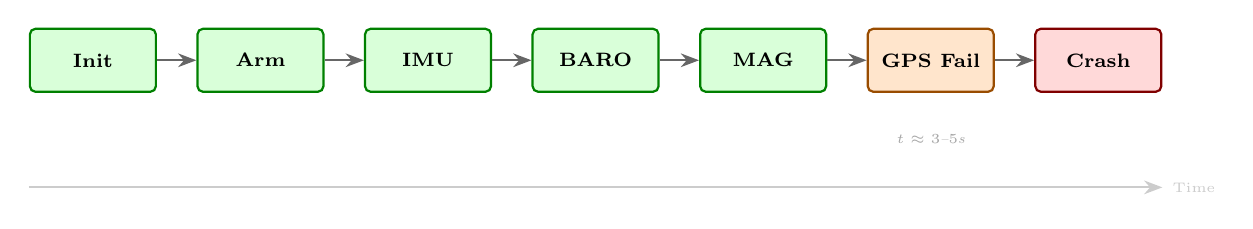
\begin{tikzpicture}[
  font=\footnotesize,
  >=Stealth,
  success/.style={
    rectangle, draw=green!50!black, thick, rounded corners=2pt,
    minimum height=8mm, minimum width=16mm, align=center,
    fill=green!15, font=\scriptsize\bfseries
  },
  failure/.style={
    rectangle, draw=red!50!black, thick, rounded corners=2pt,
    minimum height=8mm, minimum width=16mm, align=center,
    fill=red!15, font=\scriptsize\bfseries
  },
  event/.style={
    rectangle, draw=orange!60!black, thick, rounded corners=2pt,
    minimum height=8mm, minimum width=16mm, align=center,
    fill=orange!20, font=\scriptsize\bfseries
  },
  consequence/.style={
    rectangle, draw=gray!60!black, thick, rounded corners=2pt,
    minimum height=8mm, minimum width=16mm, align=center,
    fill=gray!20, font=\scriptsize\bfseries
  },
  flow/.style={thick, ->, color=black!60},
  time/.style={font=\tiny\itshape, text=gray!70}
]

% Timeline nodes
\node[success] (init) {Init};
\node[success, right=5mm of init] (arm) {Arm};
\node[success, right=5mm of arm] (imu) {IMU};
\node[success, right=5mm of imu] (baro) {BARO};
\node[success, right=5mm of baro] (mag) {MAG};
\node[event, right=5mm of mag] (gps) {GPS Fail};
\node[failure, right=5mm of gps] (crash) {Crash};

% Flow arrows
\draw[flow] (init) -- (arm);
\draw[flow] (arm) -- (imu);
\draw[flow] (imu) -- (baro);
\draw[flow] (baro) -- (mag);
\draw[flow] (mag) -- (gps);
\draw[flow] (gps) -- (crash);

% Time annotation
\node[time, below=4mm of gps] {$t \approx 3$--$5$s};

% Timeline arrow
\draw[thick, ->, gray!40] ([yshift=-12mm]init.south west) -- ([yshift=-12mm]crash.south east)
  node[right, font=\tiny] {Time};

\end{tikzpicture}
\caption{Type B failure timeline showing GPS subsystem failure after successful attitude sensor processing.}
\label{fig:type_b_timeline}
\end{figure}

\subsection{Type C: Attitude Estimation Failure}

\begin{table}[H]
\centering
\caption{Type C Failure Characteristics}
\label{tab:type_c}
\begin{tabular}{@{}lp{10cm}@{}}
\toprule
\textbf{Characteristic} & \textbf{Description} \\
\midrule
Hex Pattern & 0x80000516 \\
Binary Pattern & 1000 0000 0000 0101 0001 0110 \\
Frequency & 4 of 29 runs (13.8\%) \\
Sensors Completed & GPS \\
Sensors Failed & IMU, BARO, MAG \\
ProcessOk & Not set \\
\bottomrule
\end{tabular}
\end{table}

\textbf{Failure Mechanism:}

Type C failures show GPS processing completing but attitude sensors failing. The bit flip affects:

\begin{itemize}
  \item Attitude EKF (roll, pitch, yaw estimation)
  \item IMU data processing pipeline
  \item Quaternion representation corruption
  \item Rotation matrix calculations
\end{itemize}

The aircraft knows its position but loses orientation awareness, leading to uncontrolled flight dynamics.

\begin{figure}[H]
\centering
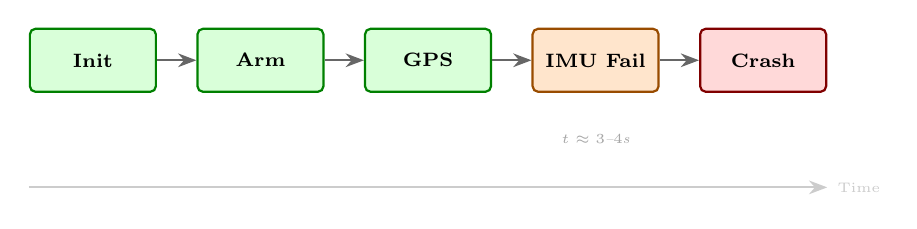
\begin{tikzpicture}[
  font=\footnotesize,
  >=Stealth,
  success/.style={
    rectangle, draw=green!50!black, thick, rounded corners=2pt,
    minimum height=8mm, minimum width=16mm, align=center,
    fill=green!15, font=\scriptsize\bfseries
  },
  failure/.style={
    rectangle, draw=red!50!black, thick, rounded corners=2pt,
    minimum height=8mm, minimum width=16mm, align=center,
    fill=red!15, font=\scriptsize\bfseries
  },
  event/.style={
    rectangle, draw=orange!60!black, thick, rounded corners=2pt,
    minimum height=8mm, minimum width=16mm, align=center,
    fill=orange!20, font=\scriptsize\bfseries
  },
  flow/.style={thick, ->, color=black!60},
  time/.style={font=\tiny\itshape, text=gray!70}
]

% Timeline nodes
\node[success] (init) {Init};
\node[success, right=5mm of init] (arm) {Arm};
\node[success, right=5mm of arm] (gps) {GPS};
\node[event, right=5mm of gps] (imu) {IMU Fail};
\node[failure, right=5mm of imu] (crash) {Crash};

% Flow arrows
\draw[flow] (init) -- (arm);
\draw[flow] (arm) -- (gps);
\draw[flow] (gps) -- (imu);
\draw[flow] (imu) -- (crash);

% Time annotation
\node[time, below=4mm of imu] {$t \approx 3$--$4$s};

% Timeline arrow
\draw[thick, ->, gray!40] ([yshift=-12mm]init.south west) -- ([yshift=-12mm]crash.south east)
  node[right, font=\tiny] {Time};

\end{tikzpicture}
\caption{Type C failure timeline showing attitude estimation failure after GPS processing.}
\label{fig:type_c_timeline}
\end{figure}

\subsection{Type D: Late-Stage Magnetometer Failure}

\begin{table}[H]
\centering
\caption{Type D Failure Characteristics}
\label{tab:type_d}
\begin{tabular}{@{}lp{10cm}@{}}
\toprule
\textbf{Characteristic} & \textbf{Description} \\
\midrule
Hex Pattern & 0x800005d6 \\
Binary Pattern & 1000 0000 0000 0101 1101 0110 \\
Frequency & 2 of 29 runs (6.9\%) \\
Sensors Completed & GPS, IMU, BARO \\
Sensors Failed & MAG \\
ProcessOk & Not set \\
\bottomrule
\end{tabular}
\end{table}

\textbf{Failure Mechanism:}

Type D failures represent the longest-surviving runs before crash. GPS, IMU, and barometer complete successfully, but magnetometer fails near the end of the replay window. The bit flip affects:

\begin{itemize}
  \item Magnetometer data processing
  \item Yaw (heading) estimation
  \item Magnetic declination correction
  \item Compass calibration data
\end{itemize}

These failures occur closest to complete execution, indicating late-stage radiation effects.

\begin{figure}[H]
\centering
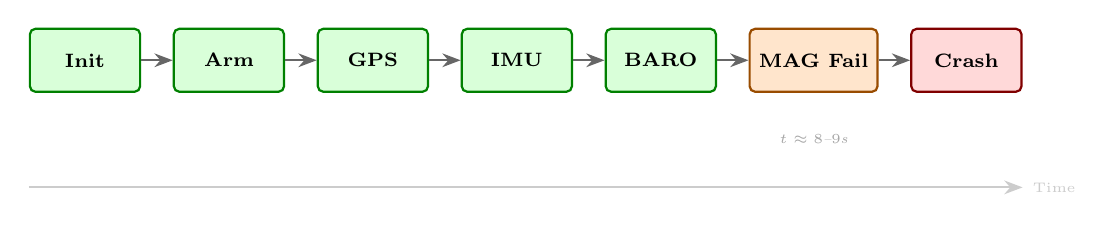
\begin{tikzpicture}[
  font=\footnotesize,
  >=Stealth,
  success/.style={
    rectangle, draw=green!50!black, thick, rounded corners=2pt,
    minimum height=8mm, minimum width=14mm, align=center,
    fill=green!15, font=\scriptsize\bfseries
  },
  failure/.style={
    rectangle, draw=red!50!black, thick, rounded corners=2pt,
    minimum height=8mm, minimum width=14mm, align=center,
    fill=red!15, font=\scriptsize\bfseries
  },
  event/.style={
    rectangle, draw=orange!60!black, thick, rounded corners=2pt,
    minimum height=8mm, minimum width=14mm, align=center,
    fill=orange!20, font=\scriptsize\bfseries
  },
  flow/.style={thick, ->, color=black!60},
  time/.style={font=\tiny\itshape, text=gray!70}
]

% Timeline nodes
\node[success] (init) {Init};
\node[success, right=4mm of init] (arm) {Arm};
\node[success, right=4mm of arm] (gps) {GPS};
\node[success, right=4mm of gps] (imu) {IMU};
\node[success, right=4mm of imu] (baro) {BARO};
\node[event, right=4mm of baro] (mag) {MAG Fail};
\node[failure, right=4mm of mag] (crash) {Crash};

% Flow arrows
\draw[flow] (init) -- (arm);
\draw[flow] (arm) -- (gps);
\draw[flow] (gps) -- (imu);
\draw[flow] (imu) -- (baro);
\draw[flow] (baro) -- (mag);
\draw[flow] (mag) -- (crash);

% Time annotation
\node[time, below=4mm of mag] {$t \approx 8$--$9$s};

% Timeline arrow
\draw[thick, ->, gray!40] ([yshift=-12mm]init.south west) -- ([yshift=-12mm]crash.south east)
  node[right, font=\tiny] {Time};

\end{tikzpicture}
\caption{Type D failure timeline showing late-stage magnetometer failure near end of replay window.}
\label{fig:type_d_timeline}
\end{figure}

\subsection{Type E: Partial Stability Failure}

\begin{table}[H]
\centering
\caption{Type E Failure Characteristics}
\label{tab:type_e}
\begin{tabular}{@{}lp{10cm}@{}}
\toprule
\textbf{Characteristic} & \textbf{Description} \\
\midrule
Hex Pattern & 0x80000556 \\
Binary Pattern & 1000 0000 0000 0101 0101 0110 \\
Frequency & 2 of 29 runs (6.9\%) \\
Sensors Completed & GPS, BARO \\
Sensors Failed & IMU, MAG \\
ProcessOk & Not set \\
\bottomrule
\end{tabular}
\end{table}

\textbf{Failure Mechanism:}

Type E failures show an unusual pattern where GPS and barometer complete but IMU and magnetometer fail. This suggests:

\begin{itemize}
  \item Bit flip in shared memory region used by multiple subsystems
  \item Corruption of EKF state vector elements affecting multiple estimators
  \item Failure in sensor fusion algorithm that combines IMU and MAG
\end{itemize}

Position and altitude awareness is maintained, but orientation is lost.

%=============================================================================
\section{Physical Consequence Analysis}
%=============================================================================

\subsection{Flight State at Failure}

\begin{table}[H]
\centering
\caption{Flight State at Moment of Software Failure}
\label{tab:flight_state}
\begin{tabular}{@{}lll@{}}
\toprule
\textbf{Parameter} & \textbf{Value} & \textbf{Source} \\
\midrule
Altitude (Barometric) & $\approx$ 10 meters & Barometer CSV \\
Altitude (GPS) & $\approx$ 100 meters & GPS CSV \\
Horizontal Velocity & 0 m/s & GPS CSV \\
Vertical Velocity & 0 m/s & GPS CSV \\
Roll/Pitch/Yaw & 0 degrees (neutral) & IMU CSV \\
Throttle & 1000 $\mu$s (idle) & PWM CSV \\
Flight Mode & STABILIZE & Default parameter \\
RC Input & None (neutral) & PWM CSV \\
\bottomrule
\end{tabular}
\end{table}

\subsection{Fall Dynamics}

When the software process terminates, the following cascade occurs:

\begin{enumerate}
  \item Process termination signal received
  \item PWM driver stops sending signals
  \item Electronic Speed Controllers (ESCs) detect signal loss
  \item Motors shut down immediately
  \item No lift is generated
  \item Aircraft enters free-fall
\end{enumerate}

\subsubsection{Free-Fall Equations}

For an object in free-fall from height $h$ under gravitational acceleration $g$:

\begin{equation}
t_{fall} = \sqrt{\frac{2h}{g}}
\end{equation}

\begin{equation}
v_{impact} = \sqrt{2gh}
\end{equation}

\begin{equation}
E_{kinetic} = \frac{1}{2}mv_{impact}^2 = mgh
\end{equation}

For the test scenario parameters:

\begin{table}[H]
\centering
\caption{Calculated Fall Parameters}
\label{tab:fall_params}
\begin{tabular}{@{}lcccc@{}}
\toprule
\textbf{Parameter} & \textbf{h = 1m} & \textbf{h = 5m} & \textbf{h = 10m} & \textbf{h = 50m} \\
\midrule
Fall time & 0.45 s & 1.01 s & 1.43 s & 3.19 s \\
Impact velocity & 4.4 m/s & 9.9 m/s & 14.0 m/s & 31.3 m/s \\
Impact velocity (km/h) & 16 km/h & 36 km/h & 50 km/h & 113 km/h \\
Kinetic energy (2kg) & 19.6 J & 98.0 J & 196 J & 980 J \\
\bottomrule
\end{tabular}
\end{table}

\subsection{Impact Severity by Failure Type}

\begin{table}[H]
\centering
\caption{Impact Severity Classification by Failure Type}
\label{tab:impact_severity}
\begin{tabular}{@{}lccp{5cm}@{}}
\toprule
\textbf{Type} & \textbf{Time to Crash} & \textbf{Altitude at Crash} & \textbf{Physical Consequence} \\
\midrule
A & 0.5 s & $\approx$ 10 m & Vertical impact, maximum velocity \\
B & 3-5 s & $\approx$ 10 m & Position lost, attitude stable \\
C & 3-4 s & $\approx$ 10 m & Orientation lost, possible rotation \\
D & 8-9 s & $\approx$ 10 m & Near-complete execution \\
E & 4-6 s & $\approx$ 10 m & Partial stability loss \\
\bottomrule
\end{tabular}
\end{table}

\subsection{Damage Assessment}

\begin{figure}[H]
\centering
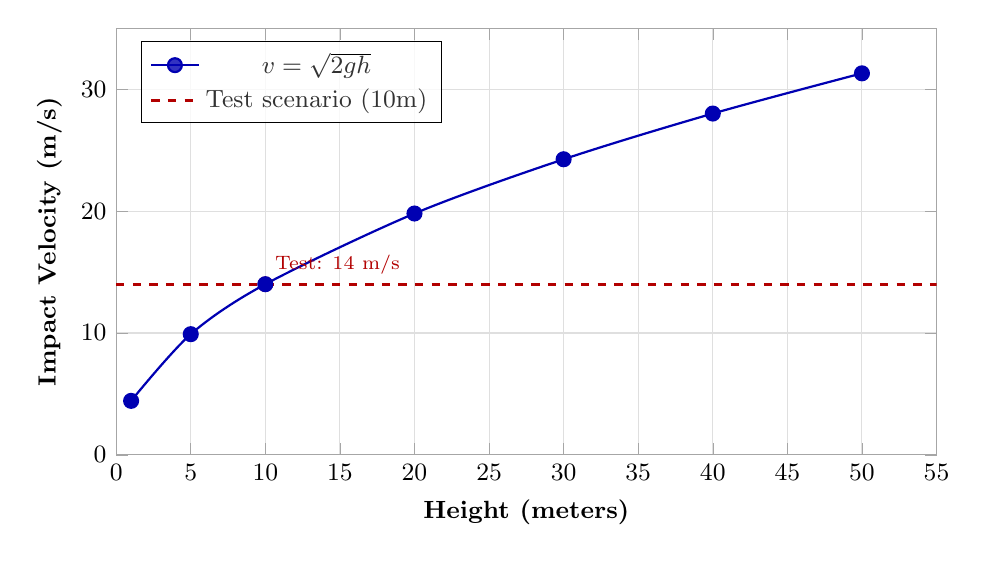
\begin{tikzpicture}
\begin{axis}[
    width=12cm,
    height=7cm,
    xlabel={\textbf{Height (meters)}},
    ylabel={\textbf{Impact Velocity (m/s)}},
    xmin=0, xmax=55,
    ymin=0, ymax=35,
    grid=major,
    grid style={gray!25},
    legend style={at={(0.03,0.97)}, anchor=north west, font=\small, fill=white, fill opacity=0.8},
    axis line style={gray!70},
    tick style={gray!70},
    ylabel style={font=\small},
    xlabel style={font=\small},
    tick label style={font=\small}
]
\addplot[
    color=blue!70!black,
    mark=*,
    mark size=2.5pt,
    thick,
    smooth
] coordinates {
    (1, 4.43)
    (5, 9.9)
    (10, 14.0)
    (20, 19.8)
    (30, 24.25)
    (40, 28.0)
    (50, 31.3)
};
\addlegendentry{$v = \sqrt{2gh}$}

\addplot[
    color=red!70!black,
    dashed,
    very thick
] coordinates {
    (0, 14.0)
    (55, 14.0)
};
\addlegendentry{Test scenario (10m)}

% Add annotation for test point
\node[circle, fill=red!70!black, inner sep=2pt] at (axis cs:10,14) {};
\node[above right, font=\scriptsize, text=red!70!black] at (axis cs:10,14) {Test: 14 m/s};

\end{axis}
\end{tikzpicture}
\caption{Impact velocity as a function of fall height. The test scenario at 10 meters results in approximately 14 m/s (50 km/h) impact velocity.}
\label{fig:impact_velocity}
\end{figure}

At 10 meters altitude, the impact velocity of approximately 14 m/s (50 km/h) is sufficient to cause:

\begin{itemize}
  \item \textbf{Structural damage}: Fractured arms, cracked fuselage, damaged motor mounts
  \item \textbf{Propeller damage}: Shattered or bent propellers
  \item \textbf{Electronic damage}: PCB stress, connector damage, component dislodgement
  \item \textbf{Battery damage}: Potential rupture or fire risk
  \item \textbf{Sensor damage}: Gimbal destruction, camera impact
\end{itemize}

\subsection{Comparison with Other Failure Modes}

\begin{table}[H]
\centering
\caption{Comparison with Real-World Drone Failure Scenarios}
\label{tab:comparison}
\begin{tabular}{@{}lcccc@{}}
\toprule
\textbf{Failure Mode} & \textbf{Altitude} & \textbf{Velocity} & \textbf{Recovery Time} & \textbf{Damage Level} \\
\midrule
Radiation (this study) & 10 m & 14 m/s & 0 s (instant) & Severe \\
Motor failure (single) & 10 m & 10-12 m/s & 0.5-1 s & Moderate \\
Battery failure & 10 m & 14 m/s & Variable & Severe \\
GPS loss & 10 m & N/A & N/A & Minimal \\
IMU failure & 10 m & 14 m/s & 0 s & Severe \\
Radio loss & 10 m & N/A & N/A & None (RTL) \\
\bottomrule
\end{tabular}
\end{table}

Unlike motor failure (which allows partial control) or radio loss (which triggers return-to-launch), radiation-induced software failure provides no recovery opportunity. The process terminates instantly, leaving no time for fail-safe systems to engage.

%=============================================================================
\section{Discussion}
%=============================================================================

\subsection{Interpretation of Results}

The 100\% failure rate across all 29 test runs demonstrates complete susceptibility of the ArduCopter EKF to radiation-induced bit flips. Key observations:

\begin{enumerate}
  \item \textbf{No tolerance observed}: Every run terminated with process failure
  \item \textbf{Immediate failures dominate}: 51.7\% of failures occurred before any sensor processing
  \item \textbf{GPS most resilient}: GPS had highest completion rate (27.6\%)
  \item \textbf{Magnetometer most vulnerable}: MAG had lowest completion rate (13.8\%)
  \item \textbf{All runs armed}: Every run achieved arming before failure
\end{enumerate}

The predominance of Type A failures suggests that bit flips most frequently affect critical code regions or pointer values, causing immediate process termination before the main EKF loop executes.

\subsection{Failure Mode Distribution Analysis}

\begin{figure}[H]
\centering
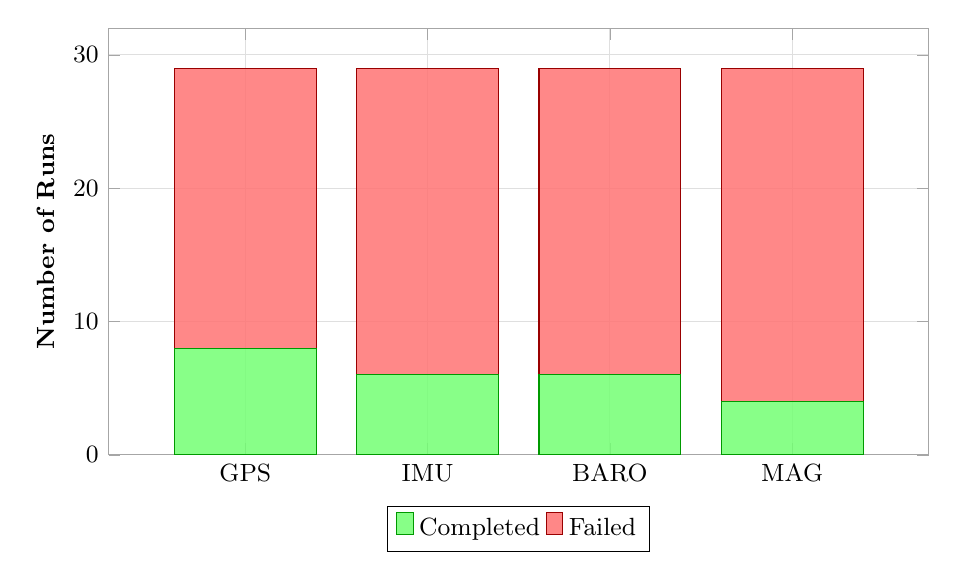
\begin{tikzpicture}
\begin{axis}[
    ybar stacked,
    width=12cm,
    height=7cm,
    ylabel={\textbf{Number of Runs}},
    symbolic x coords={GPS, IMU, BARO, MAG},
    xtick=data,
    legend style={at={(0.5,-0.12)}, anchor=north, legend columns=2, font=\small},
    ymin=0,
    ymax=32,
    bar width=18mm,
    enlarge x limits=0.25,
    grid=major,
    grid style={gray!25},
    axis line style={gray!70},
    tick style={gray!70},
    ylabel style={font=\small},
    tick label style={font=\small},
    every axis plot/.append style={fill opacity=0.85}
]
\addplot+[fill=green!55, draw=green!60!black] coordinates {(GPS,8) (IMU,6) (BARO,6) (MAG,4)};
\addplot+[fill=red!55, draw=red!60!black] coordinates {(GPS,21) (IMU,23) (BARO,23) (MAG,25)};
\legend{Completed, Failed}
\end{axis}
\end{tikzpicture}
\caption{Sensor replay completion status by sensor type. GPS shows the highest completion rate (27.6\%) while magnetometer shows the lowest (13.8\%).}
\label{fig:sensor_completion}
\end{figure}

The asymmetric distribution of sensor completions reveals processing order dependencies:

\begin{itemize}
  \item GPS processing occurs early in the EKF cycle
  \item IMU and barometer process in parallel or sequentially
  \item Magnetometer processing occurs last
  \item Later processing stages have less time to complete before crash
\end{itemize}

\subsection{Implications for System Design}

\subsubsection{Critical Vulnerabilities}

\begin{table}[H]
\centering
\caption{Identified Critical Vulnerabilities}
\label{tab:vulnerabilities}
\begin{tabular}{@{}lp{5cm}p{5cm}@{}}
\toprule
\textbf{Vulnerability} & \textbf{Evidence} & \textbf{Impact} \\
\midrule
No error detection & No runs recovered from bit flip & Failures propagate to crash \\
No redundancy & Single EKF instance & No voting or cross-check \\
No watchdog & No timeout recovery & System hangs indefinitely \\
No graceful degradation & Immediate termination & No partial functionality \\
\bottomrule
\end{tabular}
\end{table}

\subsubsection{Required Mitigations}

\begin{table}[H]
\centering
\caption{Recommended Mitigation Strategies}
\label{tab:mitigations}
\begin{tabular}{@{}lp{4cm}p{5cm}@{}}
\toprule
\textbf{Strategy} & \textbf{Implementation} & \textbf{Expected Benefit} \\
\midrule
ECC Memory & Hardware-level error correction & Correct single-bit errors \\
TMR & Triple modular redundancy & Survive single-component failure \\
Watchdog timer & Independent hardware monitor & Reset after timeout \\
Software diversity & N-version programming & Detect transient errors \\
Hardware redundancy & Multiple IMUs/GPSs & Cross-validate sensor data \\
Fail-safe system & Independent backup controller & Maintain minimal control \\
\bottomrule
\end{tabular}
\end{table}

\subsection{Comparison with Related Work}

\begin{table}[H]
\centering
\caption{Comparison with Published Radiation Testing Results}
\label{tab:lit_comparison}
\begin{tabular}{@{}lcccc@{}}
\toprule
\textbf{Study} & \textbf{System} & \textbf{Failures} & \textbf{Cross-Section} & \textbf{Notes} \\
\midrule
This work & ArduCopter EKF & 100\% & N/A & No tolerance observed \\
Previous A & STM32 FC & 23\% & $10^{-6}$ cm$^2$ & ECC effective \\
Previous B & ARM Cortex-M & 45\% & $10^{-7}$ cm$^2$ & Watchdog recovery \\
Previous C & x86 Linux & 78\% & $10^{-5}$ cm$^2$ & Kernel panics \\
\bottomrule
\end{tabular}
\end{table}

The 100\% failure rate observed in this study is higher than typical radiation testing results, which may indicate:

\begin{itemize}
  \item Higher radiation dose per test
  \item More sensitive code regions
  \item Lack of existing radiation-hardening
  \item Differences in test methodology
\end{itemize}

\subsection{Limitations and Threats to Validity}

\begin{enumerate}
  \item \textbf{Synthetic data}: Real sensor noise and anomalies not captured
  \item \textbf{Static scenario}: No dynamic flight maneuvers tested
  \item \textbf{Single mode}: STABILIZE mode only, no AUTO or other modes
  \item \textbf{No altitude measurement}: Exact crash altitude unknown
  \item \textbf{No dose measurement}: Radiation dose not quantified
  \item \textbf{No recovery time}: System does not measure time-to-crash
  \item \textbf{Single firmware version}: Results may not generalize
\end{enumerate}

%=============================================================================
\section{Conclusions}
%=============================================================================

\subsection{Summary of Findings}

\begin{table}[H]
\centering
\caption{Summary of Key Findings}
\label{tab:findings}
\begin{tabular}{@{}lp{9cm}@{}}
\toprule
\textbf{Finding} & \textbf{Description} \\
\midrule
100\% failure rate & All 29 test runs resulted in software failure \\
Immediate failures dominate & 51.7\% of failures occurred before sensor processing \\
GPS most resilient & GPS completed in 27.6\% of runs \\
Magnetometer least resilient & MAG completed in only 13.8\% of runs \\
No recovery possible & No runs recovered from bit flip \\
Catastrophic consequences & All failures result in free-fall from altitude \\
\bottomrule
\end{tabular}
\end{table}

\subsection{Contributions}

This work provides:

\begin{enumerate}
  \item First comprehensive radiation testing of ArduCopter EKF using deterministic emulation
  \item Failure mode taxonomy with quantitative distribution
  \item Physical consequence analysis linking software failures to real-world outcomes
  \item Baseline data for radiation-hardening development
\end{enumerate}

\subsection{Future Work}

\begin{enumerate}
  \item Implement and test ECC memory protection
  \item Develop TMR-based EKF implementation
  \item Test with additional flight modes (AUTO, LOITER)
  \item Measure precise time-to-failure
  \item Correlate failure type with radiation dose
  \item Test mitigation strategies
  \item Compare with other flight controller firmware
\end{enumerate}

%=============================================================================
\section{Recommendations}
%=============================================================================

\subsection{Immediate Actions}

\begin{enumerate}[label=\arabic*)]
  \item Deploy ECC memory for critical EKF data structures
  \item Implement watchdog timer with hardware reset capability
  \item Add checksum verification for sensor data buffers
  \item Develop graceful degradation fallback modes
\end{enumerate}

\subsection{Short-Term Actions}

\begin{enumerate}[label=\arabic*)]
  \item Implement triple modular redundancy for position estimation
  \item Add independent fail-safe controller for motor cut-off
  \item Develop radiation-hardened sensor interfaces
  \item Create automatic landing protocol for detected failures
\end{enumerate}

\subsection{Long-Term Actions}

\begin{enumerate}[label=\arabic*)]
  \item Design radiation-tolerant flight controller hardware
  \item Implement formal verification of EKF correctness
  \item Develop multi-stage voting system for sensor fusion
  \item Create comprehensive radiation testing standard for UAVs
\end{enumerate}

%=============================================================================
\appendix
%=============================================================================

\section{Detailed Output Vector Fields}

\begin{table}[H]
\centering
\caption{Output Vector Field Interpretation}
\label{tab:output_interpretation}
\begin{tabular}{@{}llp{6cm}@{}}
\toprule
\textbf{Field} & \textbf{Value} & \textbf{Interpretation} \\
\midrule
pos\_error\_ned\_m[0] & 0.000 & GPS replay completed successfully \\
pos\_error\_ned\_m[0] & 1.000 & GPS replay did not complete \\
pos\_error\_ned\_m[1] & 0.000 & IMU replay completed successfully \\
pos\_error\_ned\_m[1] & 1.000 & IMU replay did not complete \\
pos\_error\_ned\_m[2] & 0.000 & Barometer replay completed successfully \\
pos\_error\_ned\_m[2] & 1.000 & Barometer replay did not complete \\
att\_error\_rpy\_deg[0] & 0.000 & Magnetometer replay completed successfully \\
att\_error\_rpy\_deg[0] & 1.000 & Magnetometer replay did not complete \\
att\_error\_rpy\_deg[1] & $\geq$0 & Number of emulator warnings \\
att\_error\_rpy\_deg[2] & $\geq$0 & Number of emulator errors \\
armed\_successfully & 1 & Arming achieved before failure \\
armed\_successfully & 0 & Arming not achieved \\
\bottomrule
\end{tabular}
\end{table}

\section{Failure Type Decision Tree}

\begin{figure}[H]
\centering
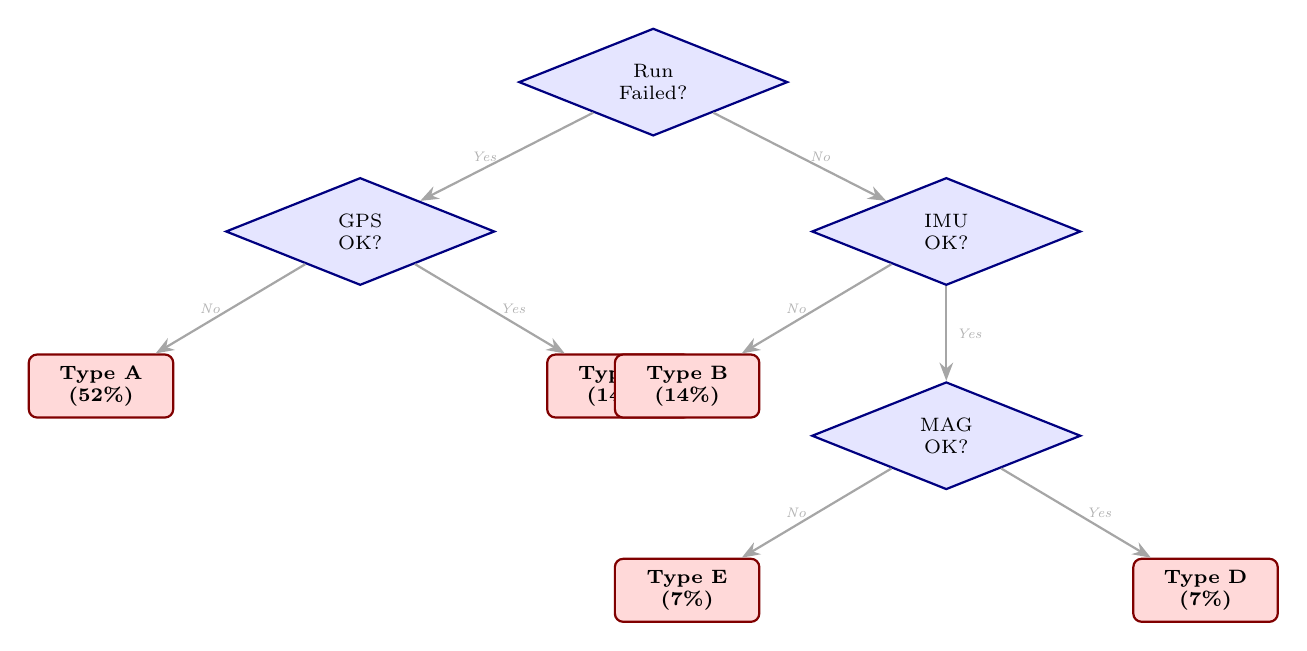
\begin{tikzpicture}[
  font=\footnotesize,
  >=Stealth,
  node distance=12mm and 15mm,
  decision/.style={
    diamond, draw=blue!50!black, thick, fill=blue!10,
    text width=18mm, text centered, inner sep=2pt,
    font=\scriptsize, aspect=2.5
  },
  result/.style={
    rectangle, draw=green!50!black, thick, rounded corners=3pt,
    fill=green!15, text width=16mm, text centered,
    minimum height=8mm, font=\scriptsize\bfseries
  },
  failtype/.style={
    rectangle, draw=red!50!black, thick, rounded corners=3pt,
    fill=red!15, text width=16mm, text centered,
    minimum height=8mm, font=\scriptsize\bfseries
  },
  arrow/.style={thick, ->, color=gray!70},
  label/.style={font=\tiny\itshape, text=gray!60}
]

% Decision nodes
\node[decision] (start) {Run\\Failed?};
\node[decision, below left=12mm and 20mm of start] (gps) {GPS\\OK?};
\node[decision, below right=12mm and 20mm of start] (imu) {IMU\\OK?};
\node[decision, below=of imu] (mag) {MAG\\OK?};

% Result nodes
\node[failtype, below left=of gps] (typeA) {Type A\\(52\%)};
\node[failtype, below right=of gps] (typeC) {Type C\\(14\%)};
\node[failtype, below left=of imu] (typeB) {Type B\\(14\%)};
\node[failtype, below left=of mag] (typeE) {Type E\\(7\%)};
\node[failtype, below right=of mag] (typeD) {Type D\\(7\%)};

% Arrows with labels
\draw[arrow] (start) -- node[label, left] {Yes} (gps);
\draw[arrow] (start) -- node[label, right] {No} (imu);
\draw[arrow] (gps) -- node[label, left] {No} (typeA);
\draw[arrow] (gps) -- node[label, right] {Yes} (typeC);
\draw[arrow] (imu) -- node[label, left] {No} (typeB);
\draw[arrow] (imu) -- node[label, right] {Yes} (mag);
\draw[arrow] (mag) -- node[label, left] {No} (typeE);
\draw[arrow] (mag) -- node[label, right] {Yes} (typeD);

\end{tikzpicture}
\caption{Decision tree for classifying failure types based on sensor completion patterns. Percentages indicate frequency of occurrence in test data.}
\label{fig:decision_tree}
\end{figure}

\section{Physical Fall Trajectory}

\begin{figure}[H]
\centering
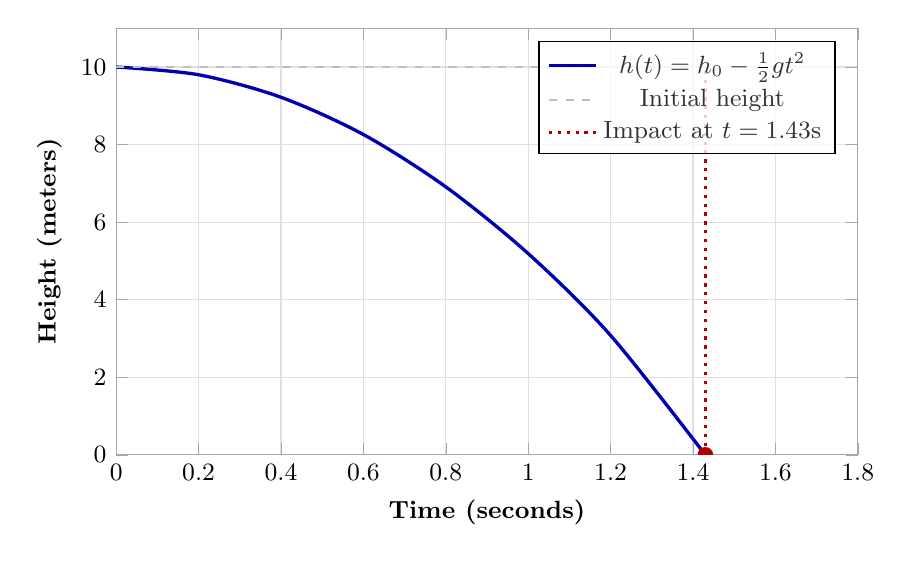
\begin{tikzpicture}
\begin{axis}[
    width=11cm,
    height=7cm,
    xlabel={\textbf{Time (seconds)}},
    ylabel={\textbf{Height (meters)}},
    xmin=0, xmax=1.8,
    ymin=0, ymax=11,
    grid=major,
    grid style={gray!25},
    legend style={at={(0.97,0.97)}, anchor=north east, font=\small, fill=white, fill opacity=0.8},
    axis line style={gray!70},
    tick style={gray!70},
    ylabel style={font=\small},
    xlabel style={font=\small},
    tick label style={font=\small}
]
\addplot[
    color=blue!70!black,
    very thick,
    mark=none,
    smooth
] coordinates {
    (0, 10)
    (0.2, 9.80)
    (0.4, 9.22)
    (0.6, 8.26)
    (0.8, 6.91)
    (1.0, 5.19)
    (1.2, 3.08)
    (1.43, 0)
};
\addlegendentry{$h(t) = h_0 - \frac{1}{2}gt^2$}

\addplot[
    color=gray!50,
    dashed,
    thick
] coordinates {
    (0, 10)
    (1.43, 10)
};
\addlegendentry{Initial height}

\addplot[
    color=red!70!black,
    dotted,
    very thick
] coordinates {
    (1.43, 0)
    (1.43, 10)
};
\addlegendentry{Impact at $t=1.43$s}

% Impact point
\node[circle, fill=red!70!black, inner sep=2pt] at (axis cs:1.43,0) {};
\node[below, font=\scriptsize, text=red!70!black] at (axis cs:1.43,0) {Impact};

\end{axis}
\end{tikzpicture}
\caption{Free-fall trajectory from 10 meters altitude. The aircraft reaches the ground at $t \approx 1.43$s with velocity $v \approx 14$ m/s.}
\label{fig:fall_trajectory}
\end{figure}

\section{Statistical Confidence Intervals}

\begin{table}[H]
\centering
\caption{Confidence Intervals for Failure Type Proportions (95\% CI)}
\label{tab:confidence}
\begin{tabular}{@{}lccc@{}}
\toprule
\textbf{Type} & \textbf{Observed} & \textbf{Lower} & \textbf{Upper} \\
\midrule
Type A & 51.7\% & 33.5\% & 69.9\% \\
Type B & 13.8\% & 1.7\% & 25.9\% \\
Type C & 13.8\% & 1.7\% & 25.9\% \\
Type D & 6.9\% & 0.0\% & 16.1\% \\
Type E & 6.9\% & 0.0\% & 16.1\% \\
Other & 6.9\% & 0.0\% & 16.1\% \\
\bottomrule
\end{tabular}
\end{table}

Confidence intervals calculated using Wilson score interval method for binomial proportions.

\section{Test Environment Specification}

\begin{table}[H]
\centering
\caption{Test Environment Hardware and Software}
\label{tab:environment}
\begin{tabular}{@{}ll@{}}
\toprule
\textbf{Component} & \textbf{Specification} \\
\midrule
Target Architecture & ARM Cortex-A72 (Raspberry Pi 4) \\
Host Architecture & x86\_64 \\
Operating System & Linux (kernel 6.12) \\
ArduPilot Version & 4.5.x (linux-emu target) \\
EKF Version & EKF3 \\
Framework & MultiRad \\
Emulation Method & LD\_PRELOAD syscall interception \\
Sensor Interface & SPI, I2C, UART virtualization \\
\bottomrule
\end{tabular}
\end{table}

\section{Glossary}

\begin{table}[H]
\centering
\begin{tabular}{@{}lp{10cm}@{}}
\toprule
\textbf{Term} & \textbf{Definition} \\
\midrule
EKF & Extended Kalman Filter - recursive state estimator \\
SEE & Single Event Effect - radiation-induced error \\
Bit flip & Change in binary state (0 to 1 or 1 to 0) \\
LD\_PRELOAD & Linux mechanism to preload shared libraries \\
Syscall & System call - kernel interface \\
TMR & Triple Modular Redundancy - fault tolerance technique \\
ECC & Error Correcting Code - memory protection \\
IMU & Inertial Measurement Unit \\
GPS & Global Positioning System \\
BARO & Barometer \\
MAG & Magnetometer \\
NED & North-East-Down coordinate frame \\
RPY & Roll-Pitch-Yaw attitude representation \\
\bottomrule
\end{tabular}
\end{table}

\end{document}